%!TEX root = mb.tex

\section{Overview}\label{sec:overview}

In this section, we present \sys's architecture, the threat model and applications supported.

\subsection{Aplomb and NEF system setup}

We recall the system setup in Aplomb and NEF setup, illustrated in Fig.~\ref{fig:sys-overview}. 
There are three parties: enterprise(s), the cloud running the middlebox, and an external site providing
some service. 
The enterprise runs a gateway (GW) which sends traffic to a middlebox (MB) running in the cloud.

There are two setups. The first setup occus when the enteprise communicates with an external site.  In this case, we have setup as in Fig.~\ref{fig:model1}.
The traffic from a client inside the enteprise passes the gateway on the way out of the enterprise. The gateway redirects this traffic to the middlebox in the cloud.
After performing various middlebox processing, MB returns the traffic to the gateway. The gateway finally sends the traffic to the external site. 


The second setup occurs when the traffic is sent between two enterprises as in Fig.~\ref{fig:model2}. This allows for a more optimized and faster layout. Each enterprise has it's own gateway.
Traffic from a client in enterprise 1 passes through the gateway of this enterprise which redirects it to the middlebox in the cloud, which after processing the traffic, it sends it to the gateway of the second enterprise which then directs it to the appropriate receiver. This setup allows for better latency, as discussed in~\cite{aplomb}.




better discuss what \sys adds here 

and returns the traffic
to the gateway which now forwards it to the external site. The answer from the external site follows the reverse direction of the
request.



\begin{figure}[t!]
\centering
\subfigure[Enterprise to external site communication]{
  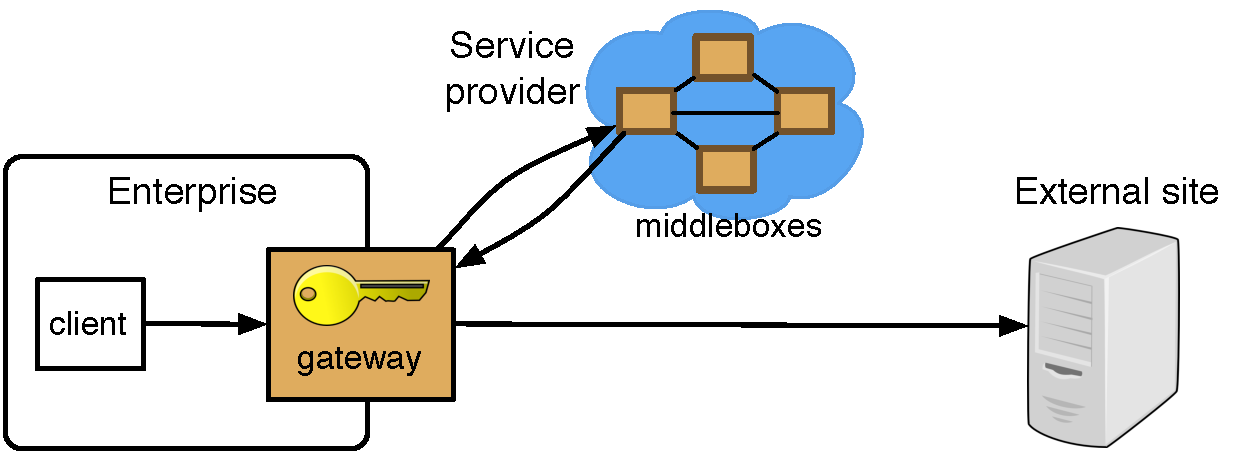
\includegraphics[width=3.3in]{fig/model_1.pdf}
  \label{fig:model1} }
%
\vfill  
\subfigure[Enterprise to enterprise communication]{
   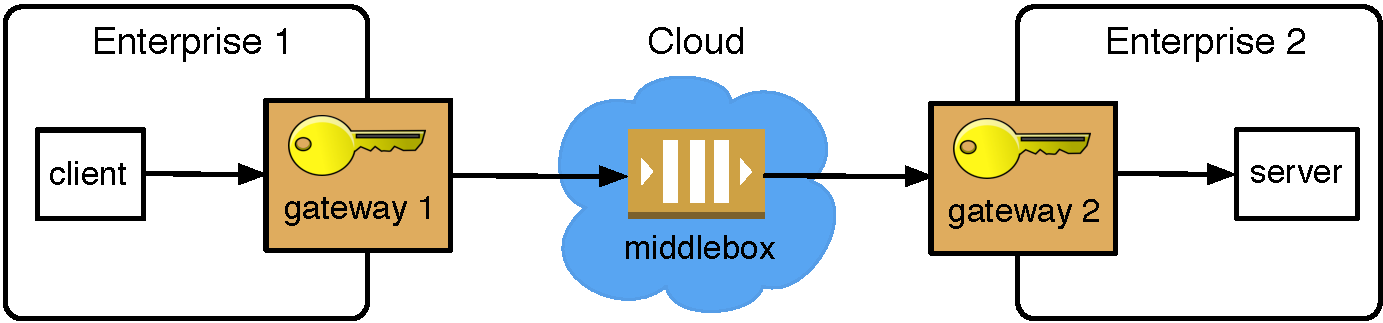
\includegraphics[width=3.1in]{fig/model_2.pdf}
     \label{fig:model2}}
%
\caption{System architecture: Aplomb and NEF system setup with \sys's encryption \label{fig:sys-overview}}
\end{figure}

\begin{itemize}
\item system architecture, figure
\item threat model
\item applications
\item use cases
\end{itemize}

\subsection{Threat model}

The goal of \sys is to protect the privacy of the traffic against an attacker at the cloud 
(cloud employee, or hacker gaining access to cloud machines). 
We consider a strong cloud attacker, one that has gained access to {\em all cloud data}.
This includes any traffic and communication the cloud receives from the 
gateway, any old logged information, cloud state, and so on. Nevertheless, we assume that 
the cloud provides good service and runs middlebox functionality correctly.  The concern is
about reading and leaking private data. 

We assume that the gateways are trusted. They do not leak information.


Some middlebox functionalities (such as intrusion detection, exfiltration detection) have a threat model
of their own about the client and the server. For example, intrusion detection assumes that 
the client or the server could misbehave and try to mount an attack, but at most one of them misbehaves 
(indeed, if both misbehave, they can send attack traffic to each other encrypted with a shared symmetric key and fundamentally
no one can detect such an attack).  We preserve all these threat models unchanged. These applications rely
on the good behavior of the middlebox to detect attacks in these threat models. Since we assume the middlebox executes
these functions correctly and \sys preserves the functionality of these middleboxes, 
these threat models are irrelevant to the protocols in \sys, and we will not discuss them again. 



\subsection{\sys overview}


The gateway encrypts
the traffic with a secret key and sends it to the middlebox in the cloud. The MB in the cloud performs various processing 
on the {\em encrypted traffic} without decrypting it (in fact, MB never gets the secret key). The result from MB is also encrypted traffic
that MB then sends to the gateway. The gateway decrypts the traffic and sends it to the external site. 
Note that any SSL connection between to the external site is maintained, but when we talk about encryption in this paper, we focus only
on \sys's added encryption. 


traffic between gateway and middlebox is encrypted

goals on the gateway

-- have a way to show that what the gateway does is generic 
   
-- somewhere we need to discuss goals regarding the gateway

-- why we choose certain operations

which app for which operation

Sys overview
- need to discuss somewhere the above goals from the gateway
A LOT OF SYSTEMS BUILDING

Sys architecture
need to spend quite some time on sys architecture

why we choose certain operations

